\section{Estimación de velocidad}
\label{cap:EstimacionVelocidad}

En este trabajo se utilizaron dos maneras para generar un modelo para determinar la velocidad, el primero se basa utilizando la formula física de la velocidad y encontrando un factor de correlación y el segundo es por el entrenamiento de modelos con los que también podemos determinar la velocidad.

\subsection{Estimar velocidad basado en factor de correlación}

Para determinar la velocidad utilizando el conjunto de datos generado por el sistema partimos de lo más sencillo utilizando la formula física para el cálculo de la velocidad, Ecuación \ref{eq:Velocidad}.

\begin{equation}
    \label{eq:Velocidad}
    Velocidad = \frac{Distancia}{Tiempo}
\end{equation}

En este caso las muestras fueron tomadas por un Radar que solo nos proporciona la velocidad en Kilómetros o en Millas, así que necesitamos convertir este valor a Metros sobre segundo, utilizando la Ecuación \ref{eq:ConvertMSKH}.

\begin{equation}
    \label{eq:ConvertMSKH}
    \frac{M}{S} = \frac{18}{5} \times \frac{K}{H}
\end{equation}

A partir que tenemos la formula física para el cálculo de la velocidad y la conversión de la velocidad en metros por segundo en lugar de kilómetros por hora, podemos definir el proceso para crear el modelo en el diagrama de flujo que se muestra en la Figura \ref{fig:CrearModeloCustom}.

\begin{figure}[H]
    \centering
    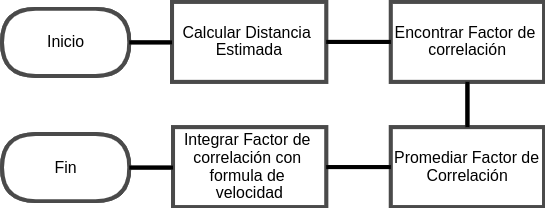
\includegraphics[width=0.9\textwidth]{Metodologia/imgs/CrearModeloCustom.png}
    \caption{Diagrama de flujo para la creacion de modelo con la formula fisica de la velocidad.}
    \label{fig:CrearModeloCustom}
\end{figure}

La Tabla \ref{tab:CaracteristicasSistema} muestra que contamos con los 3 parámetros necesarios para estimar la velocidad, sin embargo, tenemos el valor de la distancia en pixeles, por lo que tenemos que encontrar el valor de la distancia estimada utilizando los valores con los que contamos, lo cual quedaría como muestra la Ecuación \ref{eq:DistanciaEstimada}.

\begin{equation}
    \label{eq:DistanciaEstimada}
    Distancia\:Estimada = Tiempo \times Velocidad
\end{equation}

Una vez que contamos con la distancia estimada, debemos encontrar la correlación entre esta y la distancia en pixeles, con lo cual tenemos la siguiente Ecuación \ref{eq:EcuacionB}.

\begin{equation}
    \label{eq:EcuacionB}
    B = \frac{Distancia \: Estimada}{Distancia \: Pixeles}
\end{equation}

A este valor lo llamamos simplemente B, el valor de B es quien nos ayudara a calcular una velocidad estimada con respecto a la distancia y el tiempo, lo cual quedaría como muestra la Ecuación \ref{eq:VelocidadB}.

\begin{equation}
    \label{eq:VelocidadB}
    Velocidad = \frac{Distancia \: Pixeles}{Tiempo} \times B
\end{equation}

Sin embargo, esta fórmula nos serviría solo para un dato en específico generado por el sistema por lo cual debemos encontrar un valor de B que modele la gran mayoría de nuestras muestras o tener un error lo más bajo posible, para esto calculamos el valor de B para todas las muestras y calculamos el promedio de B, Ecuación \ref{eq:PromedioB}.

\begin{equation}
    \label{eq:PromedioB}
    \overline{B} = \frac{\sum B}{n}
\end{equation}

Una vez que tenemos nuestra B promedio podemos sustituirla por B en la Ecuación \ref{eq:VelocidadB} lo cual quedaría como muestra la Ecuación \ref{eq:VelocidadBPromedio}.

\begin{equation}
    \label{eq:VelocidadBPromedio}
    Velocidad = \frac{Distancia \: Pixeles}{Tiempo} \times \overline{B}
\end{equation}



\subsection{Estimar velocidad Scikit y Tensor Flow}

El proceso de creación del modelo de Scikit y Tensor Flow son el mismo, este se describe en el diagrama de flujo de la Figura \label{ref:ModeloScikitTensorFlow}.


\begin{figure}[H]
    \centering
    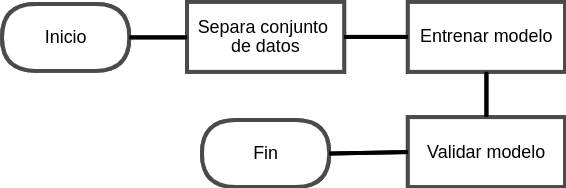
\includegraphics[width=0.9\textwidth]{Metodologia/imgs/ModeloScikitTensorFlow.png}
    \caption{Diagrama de flujo para estimar velocidad utilizando inteligencia artificial.}
    \label{fig:ModeloScikitTensorFlow}
\end{figure}


Como podemos notar el proceso para entrenar un modelo tanto en Scikit como Tensor Flow es el proceso más común utilizado. El primer paso es separar el conjunto de datos en un conjunto de entrenamiento y otro de validación normalmente esto se realiza en un porcentaje de 70\% - 30\%. Una vez separado el conjunto de datos se procede al entrenamiento utilizando la herramienta elegida, hasta que se tiene una precisión tan buena como nosotros deseemos. Por último, se utiliza el modelo con el conjunto de validación para garantizar que los resultados obtenidos sean tan buenos como en el conjunto de entrenamiento.

